\documentclass[12pt]{article}
\usepackage[hidelinks]{hyperref}    
\usepackage[all]{hypcap}
\usepackage{amssymb}
\usepackage{amsmath}
\usepackage{xcolor}
\usepackage{graphicx}
\graphicspath{{../images/lezione_2}}
% Define custom colors
\definecolor{royal_blue}{RGB}{65, 105, 225}         % Royal Blue
\definecolor{crimson_red}{RGB}{220, 20, 60}         % Crimson Red
\definecolor{goldenrod_yellow}{RGB}{218, 165, 32}   % Goldenrod Yellow

\title{\textbf{Analisi Matematica\\Insiemi e cenni di calcolo combinatorio}}
\date{19 settembre 2024}
\author{Andrea Malvezzi}
\begin{document}
\maketitle
\pagebreak
\tableofcontents
\pagebreak
\section{Definizione di sottoinsieme proprio}
Un insieme $A$ si dice sottoinsieme proprio di $B$ quando vale quanto segue:
\begin{equation}
    \text{Se } \emptyset != A \subsetneqq \label{eq:sottoinsieme_proprio}B
\end{equation}
Dove il simbolo $\subsetneqq$ sta per "inclusione stretta", ovvero:
\begin{itemize}
    \item $A \not= B$;
    \item $A \subseteq B$;
\end{itemize}
\subsection{Esempi di sottoinsiemi propri e non propri}
\begin{itemize}
    \item $A$ = $\{1, 4\}$;
    \item $B$ = $\{1, 2, 3, 4\}$;
    \item $C$ = $\{1, 2, 3, 4\}$;
\end{itemize}
Qui, $A$ è un sottoinsieme proprio di $B$ e di $C$. Tuttavia, $B$ non è sottoinsieme proprio di $C$, e viceversa.
\section{Biunivocità e invertibilità di una funzione}
Una funzione si dice biunivoca quando è sia \textit{1-1} che \textit{sv}.\\
Una funzione biunivoca è inoltre \textbf{invertibile}.
\section{Definizione di insieme numerabile}
Un insieme $\mathbb{X}$ si dice numerabile quando esiste una funzione della seguente specie:
\begin{equation}
    g: \mathbb{N} \rightarrow \mathbb{X}, \textit{g è sv} \label{eq:insieme_numerabile}
\end{equation}
\subsection{Dimostrazioni sugli insiemi numerici}
\subsubsection{$\mathbb{Z}$ è numerabile?}
Consideriamo
\[f: \mathbb{N} \rightarrow \mathbb{Z}\]
\[f(n) = \begin{cases}
    \dfrac{n}{2} \text{ se n pari} \\
    -\dfrac{n + 1}{2} \text{ se n dispari}
\end{cases}\]
Ora calcoliamo:
\begin{gather*}
    f(0) = 0 \\
    f(1) = -\dfrac{1+1}{2} = -1 \\
    f(2) = \dfrac{2}{2} = 1 \\
    \dots
\end{gather*}
Quindi $f$ è \textit{sv}, perciò $\mathbb{Z}$ è numerabile.
\pagebreak
\section{Elementi di calcolo combinatorio}
\subsection{Fattoriale di un numero}
Avendo $\mathbb{N} = \{0, 1, 2, 3, 4, ...\}$, e un $n \in \mathbb{N}$, allora si dice \textbf{fattoriale di $n$} il valore $n!$, ovvero:
\begin{equation}
    n! := 
    \begin{cases} 
        1 \cdot 2 \cdot 3 \cdot \dots \cdot (n-1) \cdot n & \text{se } n \geq 1, \\
        1 & \text{se } n = 0 
        \label{eq:fattoriale}
    \end{cases}
\end{equation}
\subsubsection{Esempio del fattoriale di un numero:}
Prendiamo come esempio il $4!$ (anche detto \textbf{4-fattoriale}).
\[4! = 1 \cdot 2 \cdot 3 \cdot 4 = 24\]
Prendiamo ora invece lo $0!$. Ricordando quanto affermato i n (\ref{eq:fattoriale}):
\[0! = 1\]
\subsection{Scomporre un numero fattoriale}\
Avendo un fattoriale $n!$, allora si può abbassare di uno $n$ e riscriverlo come $(n-1)!(n)$.
\begin{equation}
    n! = (n)(n-1)! \label{eq:scompos_fattoriale}
\end{equation} 
\subsubsection{Esempio di scomposizione numero fattoriale}
Avendo $4!$, allora potrò riscriverlo nella seguente maniera:
\[
    4! = 4 \cdot 3!
\]
Questa "proprietà" (che è in realtà una conseguenza della definizione stessa di fattoriale) sarà molto utile nelle dimostrazioni seguenti.
\subsection{Coefficiente binomiale}
Avendo due numeri tali che $n, m \in \mathbb{N} : m \leq n$, allora si dice \textbf{Coefficiente binomiale}:
\begin{equation}
    \binom{n}{m} := \dfrac{n!}{(n-m)!m!} \label{eq:coefficiente_binomiale}
\end{equation}
Dove $\dfrac{n!}{(n-m)m!}$ corrisponde a una \textbf{combinazione semplice}.
\subsubsection{Esempio di coefficiente binomiale:}
Avendo $n=3 \text{e } m=2$, allora:
\[
    \binom{3}{2} = \dfrac{3!}{2!(3-2)!} = \dfrac{6}{2} = 3
\]
\subsection{Prima proprietà del coefficiente binomiale}
\begin{equation}
    \binom{n}{k} = \binom{n}{n-k} \label{prop1_coeff_binomiale}
\end{equation}
Ovvero: ad ogni sottoinsieme di $k$ elementi corrisponde un sottoinsieme di $n-k$ elementi, per cui il loro numero è uguale.
\subsubsection{Prova algebrica}
\[
    \binom{n}{n-k} = \dfrac{n!}{[n-(n-k)]!(n-k)!} = \dfrac{n!}{k!(n-k)!} = \binom{n}{k}
\]
Per fornire un esempio concreto:
\[
    \binom{7}{2} = \dfrac{7!}{[7 - (7 - 2)]!(7-2)!} = \dfrac{7!}{5!2!} = \binom{7}{5} = \binom{7}{7-2}
\]
\subsection{Seconda proprietà del coefficiente binomiale}
\begin{equation}
    \binom{n}{k-1} + \binom{n}{k} = \binom{n+1}{k} \label{prop2_coeff_binomiale}
\end{equation}
\subsubsection{Prova algebrica}
\[
    \binom{n}{k-1} + \binom{n}{k} = \dfrac{n!}{\colorbox{goldenrod_yellow}{(n-(k-1))!}(k-1)!} + \dfrac{n!}{(n-k)!\colorbox{green}{k!}} = \dots
\]
Ora risolviamo \colorbox{goldenrod_yellow}{$-(k-1)$} e sfruttiamo (\ref{eq:scompos_fattoriale}) per scomporre \colorbox{goldenrod_yellow}{$(n-k+1)!$} in \colorbox{crimson_red}{$(n-k+1)(n-k)!$}. Inoltre, sempre applicando la medesima proprietà, scomponiamo \colorbox{green}{$k!$} in \colorbox{cyan}{$(k)(k-1)!$}.
\[
    \dots = \dfrac{n!}{(n-k+1)!(k-1)!} + \dfrac{n!}{(n-k)!k!} = \dfrac{n!}{\colorbox{crimson_red}{(n-k+1)(n-k)!}(k-1)!} + \dfrac{n!}{(n-k)!\colorbox{cyan}{k(k-1)!}} = \dots
\]
Ora raccogliamo i termini che compaiono in entrambe le frazioni:
\[
    \dots = \dfrac{n!}{(n-k)!(k-1)!}\left(\dfrac{1}{n-k+1} + \dfrac{1}{k}\right) = \dots
\]
Risolviamo le frazioni in parentesi:
\[
    \dots = \dfrac{n!}{(n-k)!(k-1)!} \cdot \dfrac{k + n -k + 1}{(n-k+1)k} = \dots
\]
Semplifichiamo la frazione di destra eliminando le due $k$ di segno opposto e moltiplichiamo tra loro le due frazioni ottenute:
\[
    \dots = \dfrac{n!(n+1)}{(n-k)!(k-1)!(n-k+1)(k)} = \dots
\]
E per finire, osserviamo come $(n-k)!$, se associato a $(n-k+1)$, permetta di ricongiungersi a una scrittura del tipo $(n-k+1)!$. La stessa cosa vale per $(k-1)!$ e $(k)$ (sempre grazie a (\ref{eq:scompos_fattoriale})).
\[
    \dots = \dfrac{(n+1)!}{(n-k+1)!k!} = \binom{n+1}{k}
\]
\subsubsection{Prova combinatoria}
Il numero di insiemi contenenti $K$ elementi componibili a partire da un insieme $N$ composto da $n+1$ elementi è pari a:
\begin{itemize}
        \item il numero di insiemi dove un certo $X_0$ è contenuto nell'insieme stesso (ovvero dove si hanno $\binom{n}{k-1}$ elementi);
    \item il numero di insiemi dove un certo $X_0$ \textbf{non} è contenuto nell'insieme stesso (ovvero dove si hanno $\binom{n}{k}$ elementi);
\end{itemize}
Che visualizzato equivale a (vedi pagina seguente):
\begin{figure}[!htb]
    \centering
    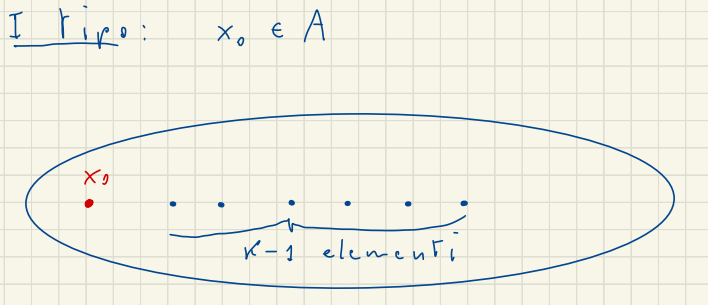
\includegraphics[width=.9\linewidth,height=.40\textheight,keepaspectratio]{prova_combinatoria_1.png} % essenzialmente resiza l'immagine
    \begin{center}
        \caption{\label{fig:prova_combinatoria_primo_caso}Primo caso descritto.} % label fuori da caption spesso non va, mettilo dentro
    \end{center}
\end{figure}
\begin{figure}[!htb]
    \centering
    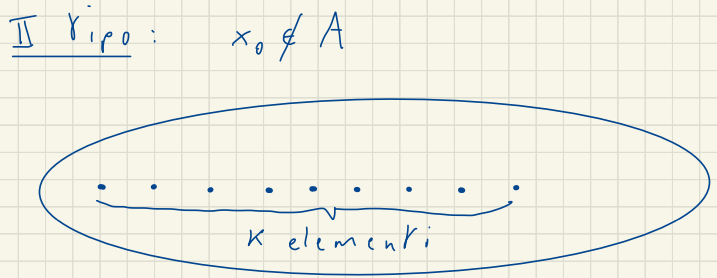
\includegraphics[width=.9\linewidth,height=.40\textheight,keepaspectratio]{prova_combinatoria_2.png} % essenzialmente resiza l'immagine
    \begin{center}
        \caption{\label{fig:prova_combinatoria_secondo_caso}Secondo caso descritto.} % label fuori da caption spesso non va, mettilo dentro
    \end{center}
\end{figure} % TODO: fix text here
Dunque in un insieme $N$ si possono avere un numero di insiemi di $K$ elementi pari alla somma di $\binom{n}{k-1}$ e di $\binom{n}{k}$.
\pagebreak
\subsection{Binomio di Newton}
Questa formula si usa per calcolare la $n$-sima potenza di un binomio in maniera semplice.
\begin{equation}
    (a+b)^n = \sum_{k=0}^{n} \binom{n}{k} \cdot a^{n-k} \cdot b^k \label{eq:binom_newton}
\end{equation}
Ma la vera comodità della formula presentata consiste nella validità delle proprietà del coefficiente binomiale precedentemente presentate.\\
(\ref{prop1_coeff_binomiale}) e (\ref{prop2_coeff_binomiale}) rimangono difatti valide anche per questa sommatoria, in quanto legata al triangolo di Tartaglia.\\
\subsubsection{Come ricavare tale formula?}
Supponiamo di voler ricavare la formula che ci permette di esprimere $(a+b)^{n}$ usando l'analisi combinatoria.\\
Prendiamo ora $c \cdot a^k \cdot b^p$, considerando che $k+p=n$. A cosa corrisponde la lettera $c$?\\
In generale si sa che $(a+b)^{n}$ corrisponda a una sommatoria di monomi del tipo: $a^{n-k}b^{k}$, con $k \in [0, n]$ considerando solo i numeri naturali.\\
Proviamo a considerare il caso più famoso di questo, ovvero il quadrato del binomio:
\[(a + b)^2 = (a + b)(a + b) = \dots = a^2 + \colorbox{yellow}{2}ab + b^2\]
Quindi la lettera $c$ corrisponde al totale dei modi con cui si può ottenere $a^{n-k}b^{k}$ in $(a + b)^{n}$
\subsubsection{Esempio di ricavo della formula prendendo $n = 4$}
Avendo $n=4$, in quanti modi posso ottenere $ab^{3}$? Bisognerà "selezionare" $b$ da tre dei quattro fattori disponibili, perciò:
\[(a + b)^4 = (a + \colorbox{yellow}{b}) \cdot (a + \colorbox{yellow}{b}) \cdot (a + \colorbox{yellow}{b}) \cdot (\colorbox{green}{a} + b)\]
Ovvero $b^3 \cdot a$. Poi, rifacendo lo stesso procedimento ma prendendo coefficienti diversi:
\[(a + b)^4 = (a + \colorbox{yellow}{b}) \cdot (a + \colorbox{yellow}{b}) \cdot (\colorbox{green}{a} + b) \cdot (a + \colorbox{yellow}{b})\]
Ovvero $b^2 \cdot a \cdot b = ab^3$.
\[(a + b)^4 = (a + \colorbox{yellow}{b}) \cdot (\colorbox{green}{a} + b) \cdot (a + \colorbox{yellow}{b}) \cdot (a + \colorbox{yellow}{b})\]
Ovvero $b \cdot a \cdot b^2 = ab^3$.
\[(a + b)^4 = (\colorbox{green}{a} + b) \cdot (a + \colorbox{yellow}{b}) \cdot (a + \colorbox{yellow}{b}) \cdot (a + \colorbox{yellow}{b})\]
Ovvero $a \cdot b^3 = ab^3$. \\
Quindi in tutto ci sono 4 modi per realizzare $ab^3$ partendo da $(a + b)^n$ con $n$ pari a $4$. Ciò significa che avendo un insieme di $4$ elementi, si avranno $4$ insiemi di $3$ elementi:
\[\binom{4}{3} = \colorbox{red}{4}\]
Ora sappiamo come risalire ad ogni tassello della formula esposta in precedenza:
\begin{equation}
    (a + b)^4 = \dots a^4b^0 + \dots a^3b + \dots a^2b^2 + \colorbox{red}{4}ab^3 + \dots a^0b^4 \label{dim:formula_binomio_newton}
\end{equation}
\subsubsection{Esempio di calcolo della \textit{n}-sima potenza di un binomio}
Per calcolare $(a+b)^n$, basterà far variare $n$ nella sommatoria presentata:
\[
    \text{Per } n=1, (a + b)^1 = \binom{1}{0}a + \binom{1}{1}b
\]
\[
    \text{Per } n=2, (a + b)^2 = \binom{2}{0}a^2 + \binom{2}{1}ab + \binom{2}{2}b^2
\]
\[
    \text{Per } n=3, (a + b)^3 = \binom{3}{0}a + \binom{3}{1}a^2b + \binom{3}{2}ab^2 + \binom{3}{3}b^3
\]
\[
    \text{etc} \dots
\]
Ora si può osservare come lo sviluppo della sommatoria presentata vada ad assumere la forma di un triangolo. Questo triangolo storicamente prende il nome di "Triangolo di Tartaglia" e permette di calcolare tutti i moltiplicatori di $a$ e di $b$ (vedi immagine sottostante).
\begin{figure}[!htb]
    \centering
    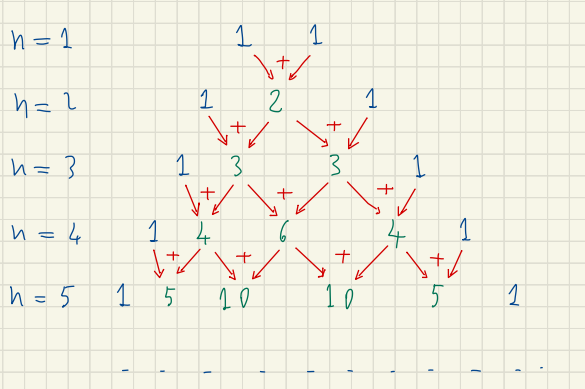
\includegraphics[width=1\textwidth, height=.7\textheight,keepaspectratio]{tartaglia.PNG} % essenzialmente resiza l'immagine
    \begin{center}
        \caption{\label{fig:tartaglia}Il triangolo di Tartaglia sviluppato fino ad n=5.} % label fuori da caption spesso non va, mettilo dentro
    \end{center}
\end{figure}
\end{document}